\documentclass{article}
\usepackage[margin=1in]{geometry}
\usepackage{amsmath,amsthm,amssymb}
\usepackage{bbm,enumerate,mathtools}
\usepackage{tikz,pgfplots}
\usepackage{chessboard}
\usepackage[hidelinks]{hyperref}
\usepackage{multicol} % Problem 35
\usepackage{xstring} % Difficulty command
\usetikzlibrary{shapes.geometric}

\newenvironment{question}{\begin{trivlist}\item[\textbf{Question.}]}{\end{trivlist}}
\newenvironment{note}{\begin{trivlist}\item[\textbf{Note.}]}{\end{trivlist}}
\newenvironment{references}{\begin{trivlist}\item[\textbf{References.}]}{\end{trivlist}}
\newenvironment{related}{\begin{trivlist}\item[\textbf{Related.}]\end{trivlist}\begin{enumerate}}{\end{enumerate}}

\newcommand\score[1]{
\pgfmathsetmacro\pgfxa{#1+1}
\tikzstyle{scorestars}=[
  star,
  star points=5,
  star point ratio=2.25,
  draw,
  inner sep=3pt,
  anchor=outer point 5
]
  \begin{tikzpicture}[baseline]
    \draw[opacity=0] (0,-0.5) rectangle (0,0.2); % Workaround for whitespace at the bottom.
    \foreach \i in {1,...,4} {
      \pgfmathparse{(\i<=#1?"yellow":"gray")}
      \edef\starcolor{\pgfmathresult}
      \draw (\i*4.5ex,0) node[name=star\i,scorestars,fill=\starcolor]  {};
    }
  \end{tikzpicture}
}

\newcommand{\difficulty}[1]{%
  \IfEqCase{#1}{%
      {1}{
        
\begin{tikzpicture}[scale=0.7, baseline=0.9mm]%
          \definecolor{slopegreen}{rgb}{0.0, 0.5, 0.0}%
          \fill[slopegreen] (0.5,0.5) circle (0.5);%
        \end{tikzpicture}%
      }%
      {2}{
        
\begin{tikzpicture}[scale=0.7, baseline=0.9mm]%
          \definecolor{slopeblue}{rgb}{0.0, 0.44, 1.00}
          \fill[slopeblue] (0,0) rectangle (1,1);%
        \end{tikzpicture}%
      }%
      {3}{
\begin{tikzpicture}[scale=0.7, baseline=0.9mm]\fill (0,0.5)--(0.5, 0)--(1,0.5)--(0.5,1)--cycle; \end{tikzpicture}}%
      {4}{
\begin{tikzpicture}[scale=0.7, baseline=0.9mm]\fill (0.25,0)--(0,0.5)--(0.25,1)--(0.5,0.5)--cycle; \fill (0.75,0)--(0.5,0.5)--(0.75,1)--(1,0.5)--cycle;\end{tikzpicture}}%
      % you can add more cases here as desired
  }[\PackageError{difficulty}{Undefined difficulty level: #1}{}]%
}%
\newcommand{\rating}[2]{\difficulty{#1}\\\score{#2}\\}


\begin{document}
\rating{4}{3}
  Suppose you choose two points on a line segment uniformly at random, defining
  three smaller line segments. The probability that these three line segments
  satisfy the triangle inequality is $\frac 14$.
  \\
  Similarly, if you choose five points on a line segment, it is conjectured that
  they can form a tetrahedron with probability $\frac 1{79}$.
\begin{figure}[ht!]
  \centering
  
\begin{tikzpicture}
    \draw[line width=5, red!50] (0,0)--(3.5,0);
    \draw[line width=5, orange!50] (3.5,0)--(6,0);
    \draw[line width=5, yellow!50] (6,0)--(9,0);
    \draw[line width=5, blue!50] (12,0)--(13.5,0);
    \draw[line width=5, purple!50] (13.5,0)--(16,0);
    \draw[line width=5, green!50] (9,0)--(12,0);
    \draw[thick]
      (0,-0.1)--(0,0.1)
      (3.5,-0.1)--(3.5,0.1)
      (6,-0.1)--(6,0.1)
      (9,-0.1)--(9,0.1)
      (12,-0.1)--(12,0.1)
      (13.5,-0.1)--(13.5,0.1)
      (16,-0.1)--(16,0.1)
    ;
  \end{tikzpicture}
  \\~\\
  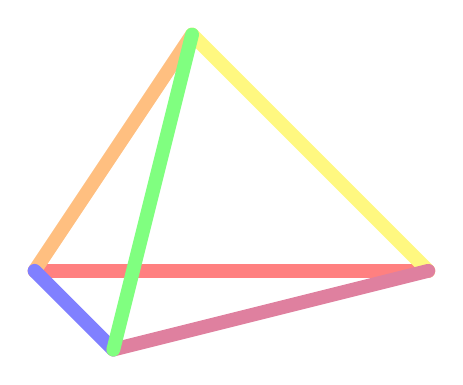
\begin{tikzpicture}
    \draw[line width=5, line cap=round, red!50] (0,0)--(5,0);
    \draw[line width=5, line cap=round, orange!50] (0,0)--(2,3);
    \draw[line width=5, line cap=round, yellow!50] (5,0)--(2,3);
    \draw[line width=5, line cap=round, blue!50] (1,-1)--(0,0);
    \draw[line width=5, line cap=round, purple!50] (1,-1)--(5,0);
    \draw[line width=5, line cap=round, green!50] (1,-1)--(2,3);
  \end{tikzpicture}
  \caption{
    An example of a partition of a line segment and the resulting tetrahedron.
  }
\end{figure}

\begin{question}
  If the line segment is split into $\frac{k(k+1)}{2}$ pieces using this
  prescription, do the resulting segments form a $k$-simplex with rational
  probability?
\end{question}

\begin{related}
  \item What if the segments form prescribed sides of the $k$-simplex? What if
    any configuration is valid?
  \item What if there are more than $\frac{k(k+1)}{2}$ pieces, what is the
    probability that there exists some subset of $\frac{k(k+1)}{2}$ of them that
    forms a $k$-simplex?
  \item What is the expected hyper-volume of such a tetrahedron?
\end{related}

\begin{references}
  \item Problem 73.
  \item Problem 78 also deals with a generalization of a Stack Exchange question.
  \item \url{https://mathoverflow.net/q/142983/104733}
\end{references}

\end{document}
